\documentclass[11pt, a4paper, norsk]{NTNUlf}
\usepackage[utf8]{inputenc}
\usepackage[T1]{fontenc}
\usepackage{float}
\usepackage{graphicx}
\usepackage{pdfpages}
\usepackage{amsthm}
\usepackage{pgfplots}
\pgfplotsset{compat=1.15}
\usepackage{mathrsfs}
\usetikzlibrary{arrows}
\usepackage{cleveref}

\setlength{\intextsep}{2.0pt plus 2.0pt minus 4.0pt}
%\setlength{\abovecaptionskip}{-15pt}

\newcommand{\R}{\mathbb{R}}

\newtheorem{lemma}{Lemma}
 
\ovingnr{2s}
\semester{Vår 2022}
\fag{MA2401 Geometri}
\institutt{Institutt for matematiske fag}
 
\begin{document}

%
 
\begin{oppgave}[1.6.3]
  Først observerer vi at det skraverte området i figuren til venstre er et kvadrat,
  siden summen av de to spisse vinklene i trekanten $\triangle ABC$ er $90^\circ$. 
  Vi ønsker å vise at det skraverte området i figuren til venstre (med areal $c^2$) 
  er like stort som det skraverte område i figuren til høyre (med areal $a^2+b^2$). 
  Begge de to store ytre kvadratene er like store, da sidene er $a+b$. Begge figurene
  inneholder fire kopier av trekanten $\triangle ABC$ (altså de hvite områdene i
  figurene). Dermed (ved å trekke fra disse fire trekantene) må de skraverte områdene
  i begge figurene være like store, altså har vi $a^2+b^2 = c^2$. 
\end{oppgave}
 
\begin{oppgave}[1.6.6]
  Merk at det er mange måter å løse disse oppgavene på, kun en av de er beskrevet her. 
  \begin{punkt}
    Konstruer to sirkler: den første skal skjære $B$ og ha sentrum i $A$; den andre 
    skal skjære $A$ og ha sentrum i $B$. Disse sirklene skjærer hverandre i to punkter. 
    Tegn en linje mellom disse to punktene. Dette er linjen vi er ute etter, altså 
    midtnormalen til linjen $\overline{AB}$. 
    \begin{figure}[H]
      \centering
      
\definecolor{qqqqff}{rgb}{0,0,1}
\begin{tikzpicture}[line cap=round,line join=round,>=triangle 45,x=1cm,y=1cm]
\clip(-4,-3.5) rectangle (7,3.5);
\draw [line width=1.2pt,domain=-7.428317161275942:7.849176681756118] plot(\x,{(-0-0*\x)/3});
\draw [line width=1.2pt] (0,0) circle (3cm);
\draw [line width=1.2pt] (3,0) circle (3cm);
\draw [line width=1.2pt] (1.5,-4.570805445724599) -- (1.5,4.135407391746856);
\begin{scriptsize}
\draw [fill=qqqqff] (0,0) circle (2pt);
\draw[color=qqqqff] (0.1831173115481543,0.1936181149389139) node {$A$};
\draw [fill=qqqqff] (3,0) circle (2.5pt);
\draw[color=qqqqff] (3.179856488450597,0.21320464550690366) node {$B$};
\end{scriptsize}
\end{tikzpicture}

      \caption{Midtnormalen til $\overline{AB}$}
    \end{figure}
  \end{punkt}

  \begin{punkt}
    Lag en sirkel med sentrum i punktet $P$ slik at sirkelen skjærer linjen $l$ i to 
    punkter -- kall disse $A$ og $B$. Konstruer midtnormalen til linjestykket 
    $\overline{AB}$, slik som i oppgave a). Denne linjen vil ved konstruksjon være 
    normal på $l$ og skjære $P$. 
    \begin{figure}[H]
      \centering
      

\definecolor{qqqqff}{rgb}{0,0,1}
\begin{tikzpicture}[line cap=round,line join=round,>=triangle 45,x=1cm,y=1cm]
\clip(-4,-3.5) rectangle (7,4);
\draw [line width=1.2pt,domain=-7.428317161275942:7.849176681756118] plot(\x,{(-0-0*\x)/3});
\draw [line width=1.2pt] (0,0) circle (3cm);
\draw [line width=1.2pt] (3,0) circle (3cm);
\draw [line width=1.2pt] (1.5,-4.443492997032665) -- (1.5,4.262719840438789);
\draw [line width=1.2pt] (1.5,1.393016028085612) circle (2.047069528497607cm);
\begin{scriptsize}
\draw [fill=qqqqff] (0,0) circle (2pt);
\draw[color=qqqqff] (0.1831173115481543,0.2436181149389139) node {$A$};
\draw [fill=qqqqff] (3,0) circle (2.5pt);
\draw[color=qqqqff] (2.779856488450597,0.21320464550690366) node {$B$};
\draw [fill=qqqqff] (1.5,3.440085556583219) circle (2.5pt);
\draw[color=qqqqff] (1.6814868999993756,3.750640760189109) node {$C$};
\end{scriptsize}
\end{tikzpicture}

    \end{figure}
  \end{punkt}

  \begin{punkt}
    Lag en sirkel med sentrum i $A$. Denne sirkelen skjærer linjestykkene $\overline{AB}$ 
    og $\overline{BC}$ i to punkter, kall disse $D$ og $E$ respektivt. Konstruer 
    midtnormalen til linjestykket $\overline{DE}$, denne linjen vil være 
    vinkelhalveringsstrålen til $\angle BAC$.
    
    \begin{figure}[H]
      \centering
      
\definecolor{qqqqff}{rgb}{0,0,1}
\begin{tikzpicture}[line cap=round,line join=round,>=triangle 45,x=1cm,y=1cm]
\clip(-4,-3.5) rectangle (7,3.5);
\draw [line width=1.2pt] (0,0)-- (5,2);
\draw [line width=1.2pt] (0,0)-- (5,-1);
\draw [line width=1.2pt] (0,0) circle (3.2310988842807022cm);
\draw [line width=1.2pt] (3,1.2) circle (1.841382833093036cm);
\draw [line width=1.2pt] (3.1683531271721495,-0.6336706254344299) circle (1.841382833093036cm);
\draw [line width=1.2pt,domain=-9.298830830518968:9.504238514751254] plot(\x,{(-0--0.16835312717214945*\x)/1.8336706254344297});
\begin{scriptsize}
\draw [fill=qqqqff] (0,0) circle (2.5pt);
\draw[color=qqqqff] (-0.17150758583571446,0.26217097192687866) node {A};
\draw [fill=qqqqff] (5,2) circle (2.5pt);
\draw[color=qqqqff] (5.253961381497465,2.1228913758859074) node {B};
\draw [fill=qqqqff] (5,-1) circle (2.5pt);
\draw[color=qqqqff] (5.253961381497465,-1.0599198414124311) node {C};
\draw [fill=qqqqff] (3,1.2) circle (2.5pt);
\draw[color=qqqqff] (3.079856488450595,1.4863291324262398) node {D};
\draw [fill=qqqqff] (3.1683531271721495,-0.6336706254344299) circle (2pt);
\draw[color=qqqqff] (3.3267554677105186,-0.905294944028564) node {E};
\end{scriptsize}
\end{tikzpicture}

      \caption{Vinkelhalveringsstrålen til $\angle BAC$}
    \end{figure}
  \end{punkt}
\end{oppgave}

\begin{oppgave}[1.6.7]

  \begin{punkt}
    Nei. Euklids postulater sier oss ingen ting om antall punkter på linjer. 
  \end{punkt}

  \begin{punkt}
    Nei. Euklids postulater sier oss ingenting dette. 
  \end{punkt}

  \begin{punkt}
    Nei. Euklids postulater sier oss at det eksisterer en linje mellom punktene, ikke at 
    det kun eksisterer \emph{én} linje. 
  \end{punkt}
\end{oppgave}

\begin{oppgave}[2.4.7]
  I Fanos geometri (se side 18 i læreboka) er punktene gitt ved symbolene $A$, $B$, 
  $C$, $D$, $E$, $F$, $G$ og linjene er de syv mengdene $\{A, B, C\}$, $\{C, D, E\}$, 
  $\{E, F, A\}$, $\{A, G, D\}$, $\{C, G, F\}$, $\{B, G, E\}$ og $\{B, D, F\}$. En 
  visualisering gitt ved følgende figur. 
  \begin{figure}[H]
    \centering
    \definecolor{qqqqff}{rgb}{0,0,1}
\begin{tikzpicture}[line cap=round,line join=round,>=triangle 45,x=1cm,y=1cm]
\clip(-1,-0.1) rectangle (7,6);
%\draw [line width=0pt] (0,0) circle (6cm);
%\draw [line width=0pt] (6,0) circle (6cm);
\draw [line width=1.2pt] (0,0)-- (3,5.196152422706632);
\draw [line width=1.2pt] (3,5.196152422706632)-- (6,0);
\draw [line width=1.2pt] (6,0)-- (0,0);
\draw [line width=1.2pt] (3,1.7320508075688772) circle (1.7320508075688772cm);
\draw [line width=1.2pt] (0,0)-- (4.5,2.598076211353316);
\draw [line width=1.2pt] (3,5.196152422706632)-- (3,0);
\draw [line width=1.2pt] (1.5,2.598076211353316)-- (6,0);
\begin{scriptsize}
\draw [fill=qqqqff] (0,0) circle (2pt);
\draw[color=qqqqff] (-0.09316146356375186,0.2132046455069031) node {$A$};
\draw [fill=qqqqff] (6,0) circle (2.5pt);
\draw[color=qqqqff] (6.076595665353041,0.2132046455069031) node {$C$};
\draw [fill=qqqqff] (3,5.196152422706632) circle (2pt);
\draw[color=qqqqff] (3.079856488450599,5.484048715456204) node {$E$};
\draw [fill=qqqqff] (1.5,2.598076211353316) circle (2pt);
\draw[color=qqqqff] (1.454174451307444,2.8182132110495433) node {$F$};
\draw [fill=qqqqff] (4.5,2.598076211353316) circle (2pt);
\draw[color=qqqqff] (4.57822607690182,2.7888334151975585) node {$D$};
\draw [fill=qqqqff] (3,0) circle (2pt);
\draw[color=qqqqff] (3.179856488450599,0.19361811493891334) node {$B$};
\draw [fill=qqqqff] (3,1.7320508075688772) circle (2pt);
\draw[color=qqqqff] (3.170063223166604,2.1) node {$G$};
\end{scriptsize}
\end{tikzpicture}

  \end{figure}
  Fanos geometri tilfredstiller det \emph{elliptiske paralellpostulatet}: for enhvær 
  linje $l$ og et punkt $P$ som ikke ligger på $l$, finnes ingen linje $m$ slik at 
  $P$ ligger på $m$ og $m$ er paralell til $l$. Grunnen er at i Fanos geometri finnes 
  det ingen paralelle linjer -- alle to linjer har et felles punkt. 
\end{oppgave}

\begin{oppgave}[2.4.10]
  Anta at vi har en modell for insidensgeometri. Av insidensaksiom 3 må modellen ha 
  minst tre punkter. Velg to av disse punktene og kall disse $A$ og $B$. Ved 
  insidensaksiom 1 ligger $A$ og $B$ på en felles linje -- kall denne $l$. Siden alle 
  linjer må inneholde tre punkter, finnes enda et punkt, $C$, på linjen $l$. 

  Fra insidensaksiom 3 må det finnes et punkt $D$ som \emph{ikke} ligger på linjen $l$. 
  Av insidensaksiom 1 bestemme punktene $A$ og $D$ en unik linje $m$, som per antagelse
  må inneholde tre punkter, kall det tredje punktet $E$. Merk at vi ikke kan ha $E=B$
  eller $E=C$, for da ville $l$ og $m$ hatt to felles punkter, og dermed vært like av 
  insidensaksiom 1. På tilsvarende måte som punkt $E$ bestemmer linjene mellom $B$ og 
  $D$ et punkt $F$, og linjen mellom $C$ og $D$ et punkt $G$. Modellen vår må dermed 
  inneholde minst syv punkter. 

  Spørsmålet er da om det eksisterer en geometri som oppfyller disse kravene, altså en 
  geometri med syv punkter som oppfyller insidensaksiomene. Vi vet at Fanos geometri 
  tilfredstiller insidensaksiomene og har syv punkter. I tillegg oppfyller Fanos geometri
  det ekstra aksiomet at alle linjer har \emph{nøyaktig} tre punkter. Altså er syv punkter
  det minste antall punkter en geometri, som oppfyller kravene, kan ha. 
\end{oppgave}

\begin{oppgave}[2.4.12]
  \begin{punkt}
    Et eksempel kan være:
    \begin{figure}[H]
      \centering
      
\definecolor{qqqqff}{rgb}{0,0,1}
\begin{tikzpicture}[line cap=round,line join=round,>=triangle 45,x=1cm,y=1cm]
\clip(-1,-1) rectangle (5,1);
\draw [line width=1.2pt,domain=-7.917980425475685:7.359513417556374] plot(\x,{(-0-0*\x)/4});
\draw[color=qqqqff] (1.973217511359173,0.5118992366687471) node[anchor=north west] {$l$};
\begin{scriptsize}
\draw [fill=qqqqff] (0,0) circle (2pt);
\draw[color=qqqqff] (0.1614634338201147,0.19361811493891334) node {$P$};
\draw [fill=qqqqff] (4,0) circle (2.5pt);
\draw[color=qqqqff] (4.157115669690038,0.2132046455069031) node {$Q$};
\draw[color=qqqqff] (-7.800461242067747,-0.012040456024979301) node {$l_{1}$};
\end{scriptsize}
\end{tikzpicture}
    \end{figure}
  \end{punkt}
  
  \begin{punkt}
    Et eksempel kan være:
    \begin{figure}[H]
      \centering
      
\definecolor{qqqqff}{rgb}{0,0,1}
\begin{tikzpicture}[line cap=round,line join=round,>=triangle 45,x=1cm,y=1cm]
\clip(-1,-1) rectangle (5,1);
\draw [line width=1.2pt,domain=-7.917980425475685:7.359513417556374] plot(\x,{(-0-0*\x)/4});
\draw[color=qqqqff] (1.973217511359173,0.5118992366687471) node[anchor=north west] {$l$};
\begin{scriptsize}
\draw [fill=qqqqff] (0,0) circle (2pt);
\draw[color=qqqqff] (0.1614634338201147,0.19361811493891334) node {$P$};
\draw [fill=qqqqff] (4,0) circle (2.5pt);
\draw[color=qqqqff] (4.157115669690038,0.2132046455069031) node {$Q$};
\draw[color=qqqqff] (-7.800461242067747,-0.012040456024979301) node {$l_{1}$};
\draw [fill=qqqqff] (2.100529960051107,-0.682879127978629) circle (2.5pt);
\draw[color=qqqqff] (2.2572222045950254,-0.47232392437273907) node {$R$};
\end{scriptsize}
\end{tikzpicture}
    \end{figure}
  \end{punkt}

  \begin{punkt}
    Et eksempel kan være:
    \begin{figure}[H]
      \centering
      

\definecolor{qqqqff}{rgb}{0,0,1}
\begin{tikzpicture}[line cap=round,line join=round,>=triangle 45,x=1cm,y=1cm]
\clip(-2,-1.5) rectangle (6,2);
\draw [line width=1.2pt,domain=-7.917980425475686:7.359513417556373] plot(\x,{(-0-0*\x)/4});
\draw [color=qqqqff](1.973217511359173,0.5118992366687471) node[anchor=north west] {$l_1$};
\draw [line width=1.2pt,domain=-7.917980425475686:7.359513417556373] plot(\x,{(-3.201593245546271--0.8003983113865677*\x)/1.9778161622208525});
\draw [line width=1.2pt,domain=-7.917980425475686:7.359513417556373] plot(\x,{(-0-0.8003983113865677*\x)/2.0221838377791475});
\draw [line width=1.2pt,domain=-7.917980425475686:7.359513417556373] plot(\x,{(-3.201593245546271-0*\x)/4});
\draw [color=qqqqff](3.277789141290547,-0.17362933321089494) node[anchor=north west] {$l_2$};
\draw [color=qqqqff](0.4588526161438042,-0.2030091290628796) node[anchor=north west] {$l_3$};
\draw [color=qqqqff](4.0298032209981045,-0.7694946388907927) node[anchor=north west] {$l_4$};
\begin{scriptsize}
\draw [fill=qqqqff] (0,0) circle (2pt);
\draw[color=qqqqff] (0.1614634338201147,0.29361811493891334) node {$P$};
\draw [fill=qqqqff] (4,0) circle (2.5pt);
\draw[color=qqqqff] (4.157115669690038,0.3132046455069031) node {$Q$};
\draw[color=black] (-7.800461242067747,-0.012040456024979301) node {$l_{1}$};
\draw [fill=qqqqff] (2.0221838377791475,-0.8003983113865677) circle (2.5pt);
\draw[color=qqqqff] (2.178876082323066,-0.4898431077806777) node {$R$};
\end{scriptsize}
\end{tikzpicture}
    \end{figure}
  \end{punkt}

\end{oppgave}
 
\begin{oppgave}[3.2.6]
  Vi definere at tre punkter $A$, $B$, $C$, på en storsirkel på $S^2$ tilfredsstiller
  $A\ast B\ast C$ dersom $s(A, C) = s(A, B) + s(B, C)$. Metrikken $s$ er definert (som
  i eksempel 3.2.12) ved at $s(A, C)$ er lengden av den korteste delbuen mellom punktene 
  $A$ og $C$ langs storsirkelen $A$ og $C$ bestemmer. Vi lar 
  $B\in \overset{\longleftrightarrow}{AC}$ bety at punktet $B$ ligger på storsirkelen 
  bestemt av $A$ og $C$. Oppgaven sier også at vi skal definere $\overline{AC}$ som 
  vanlig. Vi får $$\overline{AC} = \{A, C\}\cup \{B\vert A\ast B\ast C \} 
       = \{A, C\}\cup \{B\in \overset{\longleftrightarrow}{AC}\}\vert s(A,C) 
       = s(A, B) + s(B, C).$$

  \begin{punkt}
    Dersom $A$ og $C$ \emph{ikke} er antipodale følger det fra definisjonen over at 
    $\overline{AC}$ er den korteste delbuen mellom punktene $A$ og $C$ langs storsirkelen 
    bestemt av $A$ og $C$. Hvorfor er dette sant? Jo, at $s(A, C) = s(A, B) + s(B, C)$ 
    betyr av definisjonen av metrikken $s$ at lengden av den korteste delbuen mellom $A$ 
    og $C$ er lik summen av lengdene av de korteste delbuene mellom $A$ og $B$, og $B$ 
    og $C$. Dette gjelder hvis og bare hvis $B$ ligger på den korteste delbuen mellom $A$ 
    og $C$. Det kan være lettere å se dette ved å se på figuren under. 
    \begin{figure}[H]
      \centering
      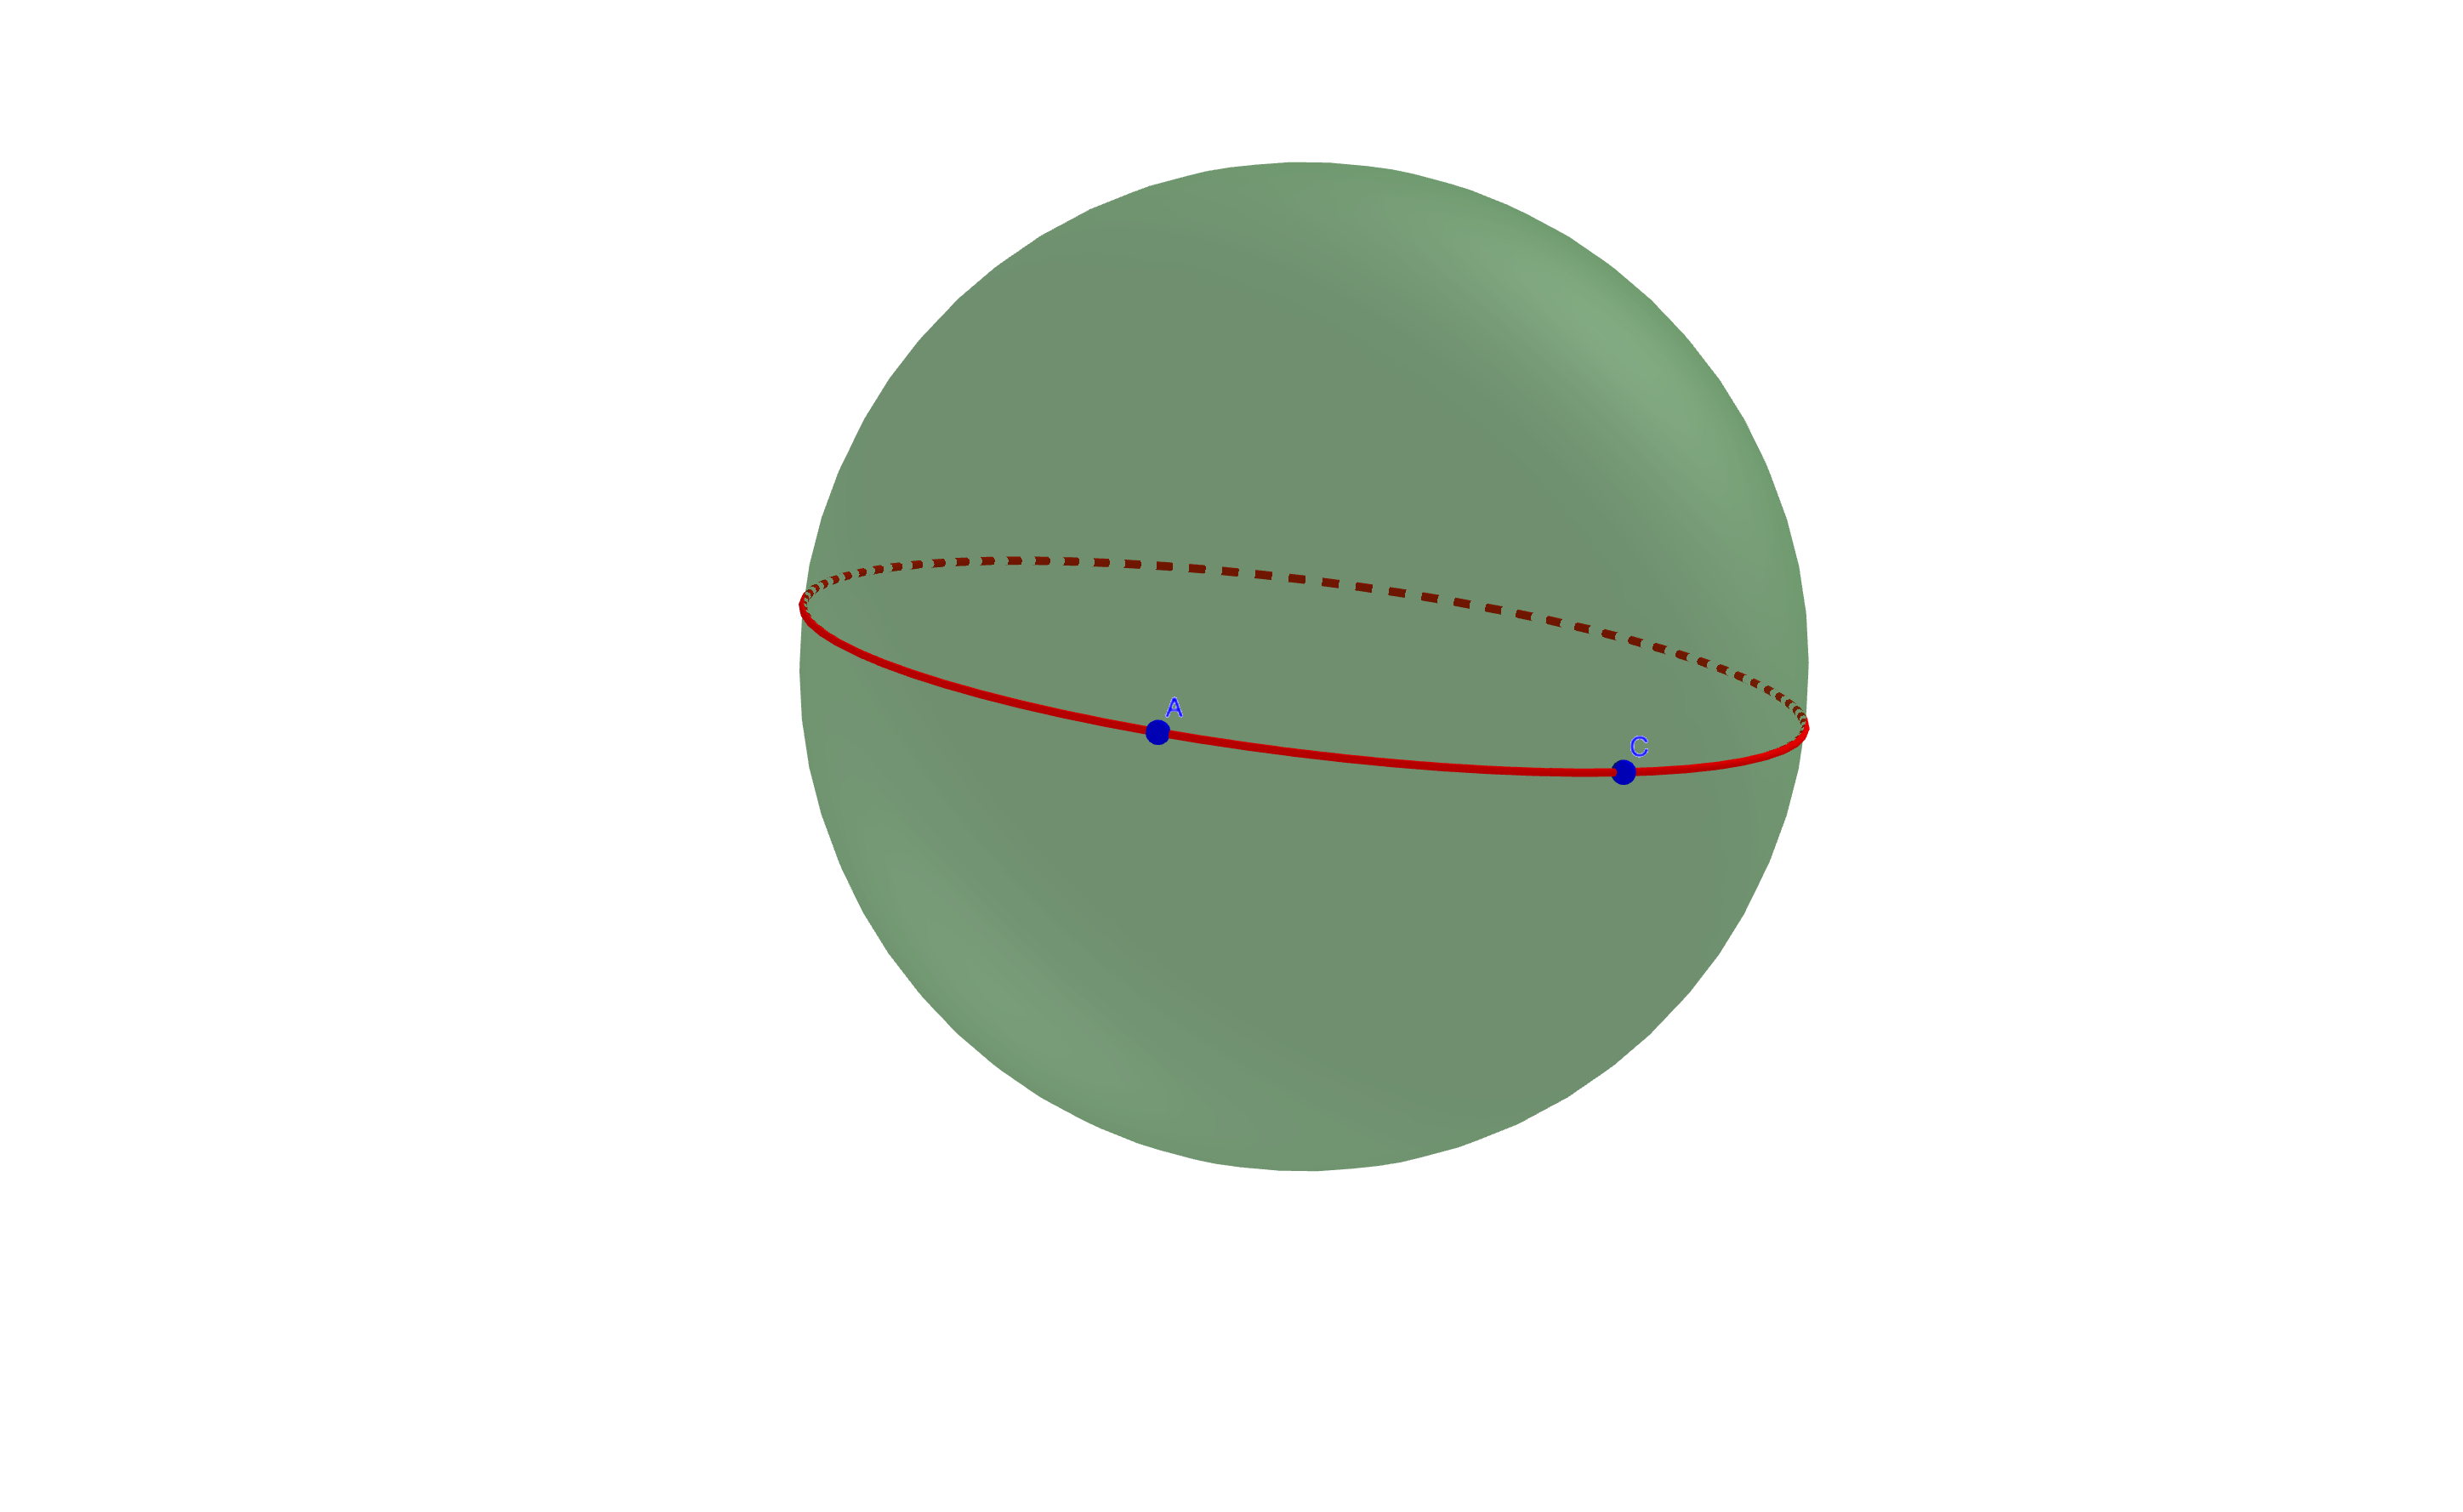
\includegraphics[trim={12cm 12cm 12cm 6cm},clip, width=\textwidth]{oving_1/326.png}
    \end{figure}
  \end{punkt}

  \begin{punkt}
    Dersom $A$ og $C$ er antipodale er $s(A, C)=\pi$ \emph{per definisjon}, ettersom $A$ 
    og $C$ ikke bestemmer en entydig storsirkel. I dette tilfellet er $\overline{AC}$ 
    hele sfæren $S^2$. Hvis vi plukker et tilfeldig punkt $B$ på sfæren, vil $A$, $B$, 
    $C$ alle tre ligge på en felles storsirkel, så det er klart at 
    $s(A,C) = \pi = s(A, B)+s(B, C)$. 
  \end{punkt}
\end{oppgave}





\begin{oppgave}[3.2.12]
  At $f:l\longrightarrow \R$ er en koordinatfunksjon betyr at 
  \begin{enumerate}
      \item $PQ=|f(P)-f(Q)|$ for alle punkter $P, Q\in l$. 
      
      \item $f$ er \emph{på}, altså at for alle $x\in \R$ finnes det et punkt $P\in l$ 
      slik at $f(P)=x$.
      
      \item $f$ er 1-til-1, altså at dersom $f(P)=f(Q)$ for to punkter $P, Q\in l$, så
      er $P=Q$. 
  \end{enumerate}
  De to siste punktene betyr at $f$ er en 1-til-1 korrespondanse. 

  \begin{punkt}
    Vi antar at $f$ er en koordinatfunksjon, og dermed tilfredstiler de tre punktene over. 
    Funksjonen er $-f$ er definert ved $(-f)(x)=-f(x)$. For å vite om dette også er en 
    koordinatfunksjon sjekker vi de tre punktene. 
    \begin{enumerate}
        \item Vi har at $|(-f)(P)-(-f)(Q)|=|-f(P)+f(Q)|=|f(P)-f(Q)|$, og siden $f$ er en 
        koordinatfunksjon vet vi at $|f(P)-f(Q)|=PQ$. Altså er $|(-f)(P)-(-f)(Q)| =PQ$. 
        
        \item Velg et tilfeldig punkt $x\in \R$. Siden $f$ er \emph{på}, finnes det et 
        punkt $P$ slik at $f(P)=-x$. Vi har da $(-f)(P) = -f(P)=-(-x)=x$, som viser at 
        også $-f$ er \emph{på}.
        
        \item La $(-f)(P)=(-f)(Q)$. Per definisjon betyr dette at $-f(P)=-f(Q)$, som igjen
        betyr at $f(P)=f(Q)$. Siden $f$ er 1-til-1 betyr dette at $P=Q$. Dermed er også $-f$
        1-til-1. 
    \end{enumerate}
  \end{punkt}

  \begin{punkt}
    Vi antar igjen at $f$ er en koordinatfunksjon. Vi sjekker om $g$ tilfredsstiller de 
    tre punktene. 
    \begin{enumerate}
        \item Vi har $|g(P)-g(Q)|=|f(P)+c - (f(Q)+c)|=|f(P)-f(Q)|$. Siden $f$ er en 
        koordinatfunksjon har vi $|f(P)-f(Q)|=PQ$, og dermed at $|g(P)-g(Q)|=PQ$. 
        \item Velg et tilfeldig punkt $x\in \R$. Siden $f$ er \emph{på} finnes det et 
        punkt $P$ slik at $f(P)=x-c$. Vi har da $g(P)=f(P)+c = x-c+c = x$. Altså er 
        $g$ også \emph{på}. 
        
        \item La $g(P)=g(Q)$. Per definisjon betyr dette at $f(P)+c=f(Q)+c$, som betyr 
        at $f(P)=f(Q)$. Siden $f$ er 1-til-1 betyr dette at $P=Q$. Dermed er også $g$
        1-til-1. 
    \end{enumerate}
  \end{punkt}

  \begin{punkt}
    Anta nå at både $f$ og $h$ er koordinatfunksjoner for $l$. For å vise at to 
    koordinatfunksjoner er like trenger vi faktisk kun å sjekke at de er like i to ulike 
    punkter. La oss se litt nærmere på dette.
    
    \begin{lemma}\label{lm:1}
      La $f$ og $h$ være koordinatfunksjoner for en linje $l$. Dersom $f(P)=h(P)$ og 
      $f(Q)=h(Q)$ for to punkter $P\neq Q$, så er $f(A)=h(A)$ for alle $A\in l$. 
    \end{lemma}

    \begin{proof}
      Anta at $f(P)=h(P)$ og $f(Q)=h(Q)$ der $P\neq Q$. Siden $P\neq Q$ har vi $f(P)\neq f(Q)$.
      Vi kan anta uten ta av generalitet at $f(P)< f(Q)$. La $A\in l$ være et punkt. Vi ønsker 
      å vise at $f(A)=h(A)$. Fra korollar 3.2.19 vet vi at dersom tre ulike punkter ligger på en
      linje, så ligger et av dem mellom de to andre. Vi har nå tre punkter: $P$, $Q$, $A$, og 
      disse kan være i tre konfigurasjoner: $P\ast A\ast Q$, $P\ast Q\ast A$ og $A\ast P\ast Q$. 
      Vi sjekker at $f(A)=h(A)$ i alle tre tilfellene. 
      \begin{enumerate}
        \item $P\ast A\ast Q$: Av teorem 3.2.17 har vi at $f(P)<f(A)<f(Q)$, og fra 
        linjalpostulatet er $$ AQ = |f(Q)-f(A)| = f(Q)-f(A), $$ der vi har fjernet 
        absoluttverditegnet ettersom $f(A)<f(Q)$. Vi har da $f(A)=f(Q)-AQ$. På samme måte får vi 
        $h(A)=h(Q)-AQ$. Dermed har vi $$ f(A)=f(Q)-AQ = h(Q)-AQ = h(A), $$ siden vi har antatt 
        at $f(Q)=h(Q)$. 
    
        \item $P\ast Q\ast A$: De to følgende punktene er så og si helt like som det over, men 
        vi skriver de ut for kompletthets skyld. 
    
        Fra teorem 3.2.17 vet vi at $f(P)<f(Q)<f(A)$, og fra linjalpostulatet er 
        $$ AQ = |f(A)-f(Q)| = f(A)-f(Q), $$ der vi igjen har fjernet absoluttverditegnet siden 
        $f(Q)<f(A)$. Vi har da $f(A)=f(Q)+AQ$. På samme måte får vi $h(A)=h(Q)+AQ$. Dermed har 
        vi $$ f(A)=f(Q)+AQ = h(Q)+AQ = h(A), $$ siden vi har antatt at $f(Q)=h(Q)$. 
    
        \item $A\ast P\ast Q$: Fra teorem 3.2.17 vet vi at $f(A)<f(P)<f(Q)$, og fra 
        linjalpostulatet er $$ AP = |f(P)-f(A)| = f(P)-f(A), $$ der vi igjen har fjernet 
        absoluttverditegnet siden $f(A)<f(P)$. Vi har da $f(A)=f(P)-AP$. På samme måte får 
        vi $h(A)=h(P)+AP$. Dermed har vi $$ f(A)=f(P)-AP = h(P)-AP = h(A), $$ siden vi har 
        antatt at $f(P)=h(P)$. 
      \end{enumerate}
    \end{proof}
    

    Ok, la oss vende tilbake til den faktiske oppgaven. Siden $f$ er en koordinatfunksjon vet 
    vi at det er \emph{på}. Dermed kan vi finne punkter $P$ og $Q$ slik at $f(P)=0$ og $f(Q)=1$.
    Fra linjalpostulatet har vi dermed at $PQ=f(Q)-f(P)=1$. Vi har to muligheter for $h$, enten 
    er $h(P)<h(Q)$, eller så er $h(Q)<h(P)$. Vi ser på den første muligheten først. 

    Anta at $h(P)< h(Q)$. Vi påstår at for en hver $A\in l$ så er $h(A)=f(A)+c$, der $c=h(P)$. Siden 
    $f$ er en koordinatfunksjon vet vi fra b) at funksjonen gitt ved $f(P)+c$ også er en 
    koordinatfunksjon. Fra \cref{lm:1} trenger vi kun å vise at $h(P)=f(P)+c$ og $h(Q)=f(Q)+c$ for 
    å bevise påstanden vår. Vi har $$f(P)+c = f(P)+h(P) = 0+ h(P) = h(P)$$ og 
    \begin{align*}
        f(Q)+c 
        &= f(Q)+h(P) \\
        &= f(Q)+(h(Q)-PQ) \\
        &= h(Q) + (f(Q)-PQ) \\
        &= h(Q),
    \end{align*}
    ettersom $f(Q) = 1 = PQ$. Den andre av likhetene over får vi fra linjalpostulatet. 

    Anta nå at $h(Q)<h(P)$. Vi påstår nå at $h(A)=-f(A)+c$, der igjen $c=h(P)$, for alle $A\in l$.
    Beviset for at dette er sant er helt analogt til det over. Altså, vi sjekker om de er like for 
    $P$ og $Q$, noe som ved \cref{lm:1} betyr at de må være like. Vi har 
    $$h(P)=0+h(P)=-f(P)+c,$$ da $f(P)=0$. Vi har også 
    \begin{align*}
        -f(Q)+c 
        &= -f(Q)+h(P) \\
        &= -f(Q)+(h(Q)+PQ) \\
        &= h(Q) + (PQ-f(Q)) \\
        &= h(Q),
    \end{align*}
    ettersom $f(Q) = 1 = PQ$. Den andre av likhetene over får vi igjen fra linjalpostulatet. 
  \end{punkt}
\end{oppgave}

\begin{oppgave}[3.2.15]
  Oppgaver ber oss om å vise at to mengder er like, altså at 
  $$\overrightarrow{AB} = \{P\in l | f(P)\geq 0\}.$$
  For å vise dette viser vi to ting: først, dersom $P\in \overrightarrow{AB}$ så er $f(P)\geq 0$,
  så, dersom $f(P)\geq 0$ så er $P\in \overrightarrow{AB}$. 
    
  Anta dermed at $P\in \overrightarrow{AB}$. Da har vi enten $P=A$, $P=B$, $A\ast P\ast B$ eller
  $A\ast B\ast P$. Dersom $P=A$ har vi fra beskrivelsen av funksjonen $f$ at $f(P)=0$ og dersom 
  $P=B$ har vi $f(P)>0$. Dersom $A\ast P\ast B$ har vi dermed fra teorem 3.2.17 i boka at 
  $f(A)< f(P)<f(B)$, og dermed at $f(P)\geq 0$. Siste mulighet er at $A\ast B\ast P$, som igjen 
  fra teorem 3.2.17 betyr at $f(A)<f(B)<f(P)$. Alle mulighetene gir oss $f(P)\geq 0$, så vi har 
  vist den første delen. 

  Anta nå at vi har $f(P)\geq 0$. Hvis $f(P)=0$ så har vi $f(A)=f(P)$. Siden $f$ er en-til-en vet 
  vi at dette betyr at $A=P$. Det tilsvarende gjelder dersom $f(P)=f(B)$. I begge tilfeller er
  $P\in \overrightarrow{AB}$. Vi har da to tilfeller igjen, $f(A)<f(P)<f(B)$ og $f(A)<f(B)<f(P)$. 
  Fra teorem 3.2.17 får vi da respektivt at $A\ast P\ast B$ og $A\ast B\ast P$. Dermed er 
  $P\in \overrightarrow{AB}$. 
\end{oppgave}

\begin{oppgave}[3.2.22]
  Vi skal vise at dersom $\overline{AB} = \overline{CD}$, så er enten $A=C$ og $B=D$ eller $A=D$
  og $B=C$. Vi bemerker oss først at $\overleftrightarrow{AB} = \overleftrightarrow{CD}$ ettersom 
  $C$ og $D$ begge ligger på linjen $\overleftrightarrow{AB}$. 

  La nå $f:\overleftrightarrow{AB}\longrightarrow \R$ være en koordinatfunksjon. Vi kan anta uten 
  tap av generalitet at $f(A)<f(B)$ og $f(C)<f(D)$. Fra teorem 3.2.17 får vi to likheter:
    
  $$ \overline{AB}=\{ P|f(A)\leq f(P)\leq f(B) \} $$
  $$ \overline{CD}=\{ P|f(C)\leq f(P)\leq f(D) \} .$$
    
  Siden vi har antatt at $\overline{AB}=\overline{CD}$ vet vi at $C\in \overline{AB}$. Fra den 
  første likheten får vi da at $f(A)\leq f(C)$. Vi vet også at $A\in \overline{CD}$, som fra den 
  andre likheten gir oss $f(C)\leq f(A)$. Siden $f(C)$ er både mindre og større enn $f(A)$ må vi 
  ha $f(A)=f(C)$. Siden $f$ er en-til-en betyr dette at $A=C$. 

  Helt tilsvarende får vi at $B=D$. Merk at mulighetene $A=D$ og $B=C$ forsvant da vi anto at 
  $f(A)<f(B)$ og $f(C)<f(D)$. Snur vi på disse ulikhetene får vi isteden $A=D$ og $B=C$. 
\end{oppgave}

\begin{oppgave}[3.2.24.d)]
  Vi skal vise at $\overline{AB}\cap \overline{BC} = \{B\}$. Siden $A, B, C$ er kolineære finnes en 
  linje $l$ som de alle ligger på. La $f:l\longrightarrow \R$ være en koordinatfunksjon for $l$. 
  Ettersom $B$ ligger mellom $A$ og $C$ vet vi fra teorem 3.2.17 at enten $f(A)<f(B)<f(C)$ eller 
  $f(A)>f(B)>f(C)$. Vi antar $f(A)<f(B)<f(C)$. Beviset vil være helt tilsvarende dersom vi isteden
  antar den andre ulikheten. Fra teorem 3.2.17 får vi to likheter

  $$ \overline{AB}=\{P|f(A)\leq f(P)\leq f(B)\} $$
  $$ \overline{BC})\{P|f(B)\leq f(P)\leq f(C)\} .$$

  Dersom vi tar et punkt $Q\in \overline{AB}\cap \overline{BC}$ må vi fra de to likhetene ha
  $ f(A)\leq f(Q)\leq f(B)$ og $f(B)\leq f(Q)\leq f(C)$. Siden $f(Q)$ er både mindre og større enn 
  $f(B)$ må vi ha $f(Q)=f(B)$. Siden $f$ er en-til-en betyr dette at $Q=B$. 
\end{oppgave}

\begin{oppgave}[3.3.1]
  La $X$ og $Y$ være to konvekse mengder. Vi velger oss to punkter $A$ og $B$ i snittet $X\cap Y$. 
  Dersom vi klarer å vise at linjen $\overline{AB}\subset X\cap Y$, så har vi vist at $X\cap Y$ også 
  er en konveks mengde. 

  Ettersom $A, B\in X\cap Y$ må vi ha $A\in X$, $A\in Y$, $B\in X$ og $B\in Y$. Siden $X$ og $Y$ er 
  konvekse mengder vet vi da at linjen $\overline{AB}\subset X$ og $\overline{AB}\subset Y$. Siden 
  linjen ligger i både $X$ og $Y$ ligger den også per definisjon i snittet av mengdene. Dermed har 
  vi $\overline{AB}\subset X\cap Y$, som var det vi ville vise. 

  Under har vi tegnet et eksempel av to disjunkte konvekse mengder (to disker) $X$ og $Y$. Som vi 
  enkelt kan se, er ikke unionen av disse en konveks mengde. Velg to punkter $A\in X$ og $B\in Y$. 
  Siden $X$ og $Y$ er disjunkte er ikke linjen $\overline{AB}$ inneholdt i $X\cup Y$. Dermed er 
  ikke unionen konveks. 

  \begin{figure}[H]
    \centering
    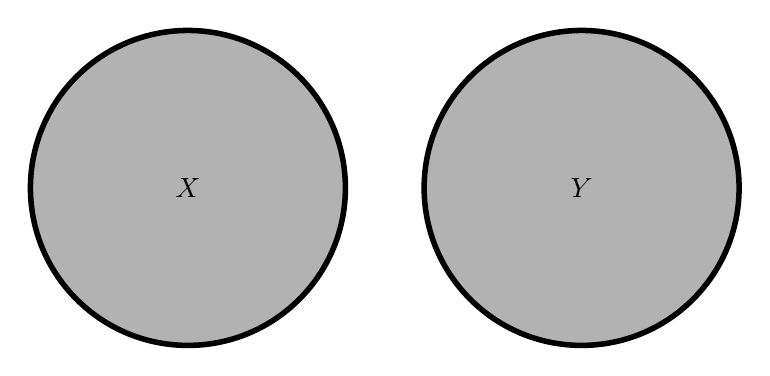
\begin{tikzpicture}
    \draw[fill, black!30] (-2,0) circle (2cm);
    \draw[fill, black!30] (3,0) circle (2cm);
    \draw[black, line width=2pt] (-2,0) circle (2cm);
    \draw[black, line width=2pt] (3,0) circle (2cm);
    \node at (-2,0) {$X$};
    \node at (3,0) {$Y$};
\end{tikzpicture}
  \end{figure}
  
  Vi har to måter å tenke på at den tomme mengden er en konveks mengde. Per definisjon inneholder 
  ikke den tomme mengden noen punkter. Dette betyr at for alle punkter (nettopp ingen) i $\emptyset$ 
  så er linjen mellom de inneholdt i $\emptyset$. Dermed tilfredstiller $\emptyset$ trivielt 
  definisjonen av å være konveks. Vi har i starten av oppgaven også vist at snittet av to konvekse 
  mengder er igjen konvekst. Så, dersom vi tar to disjunkte mengder (for eksempel de vi tegnet over)
  så vil snittet av disse være konvekst. Dette snittet er jo den tomme mengden, så den må da være 
  konveks. 
\end{oppgave}

\begin{oppgave}[3.3.2]
  \begin{itemize}
    \item $\{A\}$: I denne mengden har vi kun ett punkt, nemlig $A$. Så det eneste 
    linjestykket vi har er $\overline{AA}$. Per definisjon har vi 
    $$ \overline{AA} = \{A, A\}\cup \{P|A\ast P\ast A\} = \{A\}. $$
    Ettersom $\{A\}\subseteq \{A\}$ er mengden konveks. 

    \item $\overline{AB}$: La $C$ og $D$ være to punkter i $\overline{AB}$. For at $\overline{AB}$ 
    skal være konvekst må vi vise at linjestykket $\overline{CD}$ er inneholdt i $\overline{AB}$. 
    
    Punktene $A$, $B$, $C$ og $D$ ligger alle på linjen $\overleftrightarrow{AB}$. La 
    $f:\overleftrightarrow{AB}\longrightarrow \R$ være en koordinatfunksjon, som vi fra teorem 
    3.2.16 kan anta at oppfyller $f(A)=0$ og $f(B)>0$. Vi antar videre uten tap av generalitet at 
    $f(C)<f(D)$. Fra teorem 3.2.17 får vi to likheter

    $$ \overline{AB}=\{P|f(A)\leq f(P)\leq f(B)\} $$
    $$ \overline{CD}=\{P|f(C)\leq f(P)\leq f(D)\} .$$

    Siden $C, D\in \overline{AB}$ vet vi dermed at $f(A)\leq f(C)\leq f(D)\leq f(B)$. Dette betyr 
    også at for et hvert punkt $P\in \overline{CD}$ så har vi $f(A)\leq f(P)\leq f(B)$. Fra teorem
    3.2.17 vet vi da at $A\ast P\ast B$, som vil si at $P\in \overline{AB}$. Dermed har vi 
    $\overline{CD}\subseteq \overline{AB}$.  

    \item $\overrightarrow{AB}$: Som over lar vi $f:\overleftrightarrow{AB}\longrightarrow \R$ være
    en koordinatfunksjon slik at $f(A)=0$ of $f(B)>0$. Velg to punkter $C, D \in \overrightarrow{AB}$
    med $f(C)<f(D)$. Vi vil vise at $\overline{CD}\subset \overrightarrow{AB}$. 
    
    Siden $C, D\in \overrightarrow{AB}$ vet vi at $f(C)\geq 0$ og $f(D)\geq 0$. Fra teorem 3.2.17
    får vi likheten

    $$ \overline{CD} = \{P| f(C)\leq f(P)\leq f(D)\},$$

    som betyr at $f(P)\geq f(C)\geq 0$ for alle punkter $P\in \overline{CD}$. Siden 
    $\overrightarrow{AB} = \{P|0\leq f(P)\}$ får vi at $P\in \overleftrightarrow{AB}$ for alle 
    punkter $P\in \overline{CD}$, som betyr at $\overline{CD}\subset \overrightarrow{AB}$. 

    \item $\overleftrightarrow{AB}$: Velg to punkter $C$ og $D$ på $\overleftrightarrow{AB}$. Vi vil
    vise at $\overline{CD}\subset \overleftrightarrow{AB}$. 

    For et punkt $P\in \overline{CD}$ har vi enten $P=C$, $P=D$ eller $C\ast P\ast D$. I de to 
    første tilfellene har vi åpenbart $P\in \overleftrightarrow{AB}$. Dersom $C\ast P\ast D$ så må 
    $C$, $P$ og $D$ ligge på en felles linje $l$. Siden to punkter ligger på en \emph{unik} linje, 
    og $C$ og $D$ ligger på både $l$ og $\overleftrightarrow{AB}$ må vi ha $l=\overleftrightarrow{AB}$.
    Dermed har vi $P\in \overleftrightarrow{AB}$ som betyr at 
    $\overline{CD}\subset \overleftrightarrow{AB}$, som var det vi ville vise. 

  \end{itemize}
\end{oppgave}

\begin{oppgave}[3.3.4]
  \begin{punkt}
    Vi må vise at modellen tilfredstiller alle punktene i aksiom 3.3.2. Vi tolker her storsirkel som
    linje og halvsfære som halvplan. Det er klart at en storsirkel $l$ deler sfæren inn i to halvsfærer
    $H_1$ og $H_2$, og at disse er ikke-tomme og disjunkte. 

    Vi vil vise at $H_1$ og $H_2$ er konvekse. Anta at $A$ og $B$ er to punkter i $H_1$. Vi må altså 
    vise at linjestykket $\overline{AB}\subset H_1$. Merk at siden $A$ og $B$ ligger i samme halvsfære
    kan de ikke være antipodale. Dermed kan vi bruke (som vist i øving 1, oppgave 3.2.6(a)) at
    $\overline{AB}$ er den korteste delbuen mellom $A$ og $B$ langs den unike storsirkelen bestemt av 
    $A$ og $B$. Denne delbuen ligger i $H_1$, så $H_1$ er en konveks mengde. Tilsvarende viser at $H_2$
    er konveks. 

    La $C\in H_1$ og $D\in H_2$ har vi to muligheter: 
    \begin{enumerate}
      \item $C$ og $D$ er antipodale. Dette vil si at $\overline{CD} = S^2$, som vil si at
      $\overline{CD}\cap l = l$. 

      \item $C$ og $D$ er ikke antipodale. Siden $C$ og $D$ ligger i forskjellige halvsfærer vil 
      enhver sti fra $C$ til $D$ krysse $l$, spesielt vil dette gjelde for $\overline{CD}$. 
    \end{enumerate}

    I begge tilfellene er snittet $\overline{CD}\cap l\neq \emptyset$. Oppgaven kan oppsummeres med
    følgende figur: 
    \begin{figure}[H]
      \centering 
      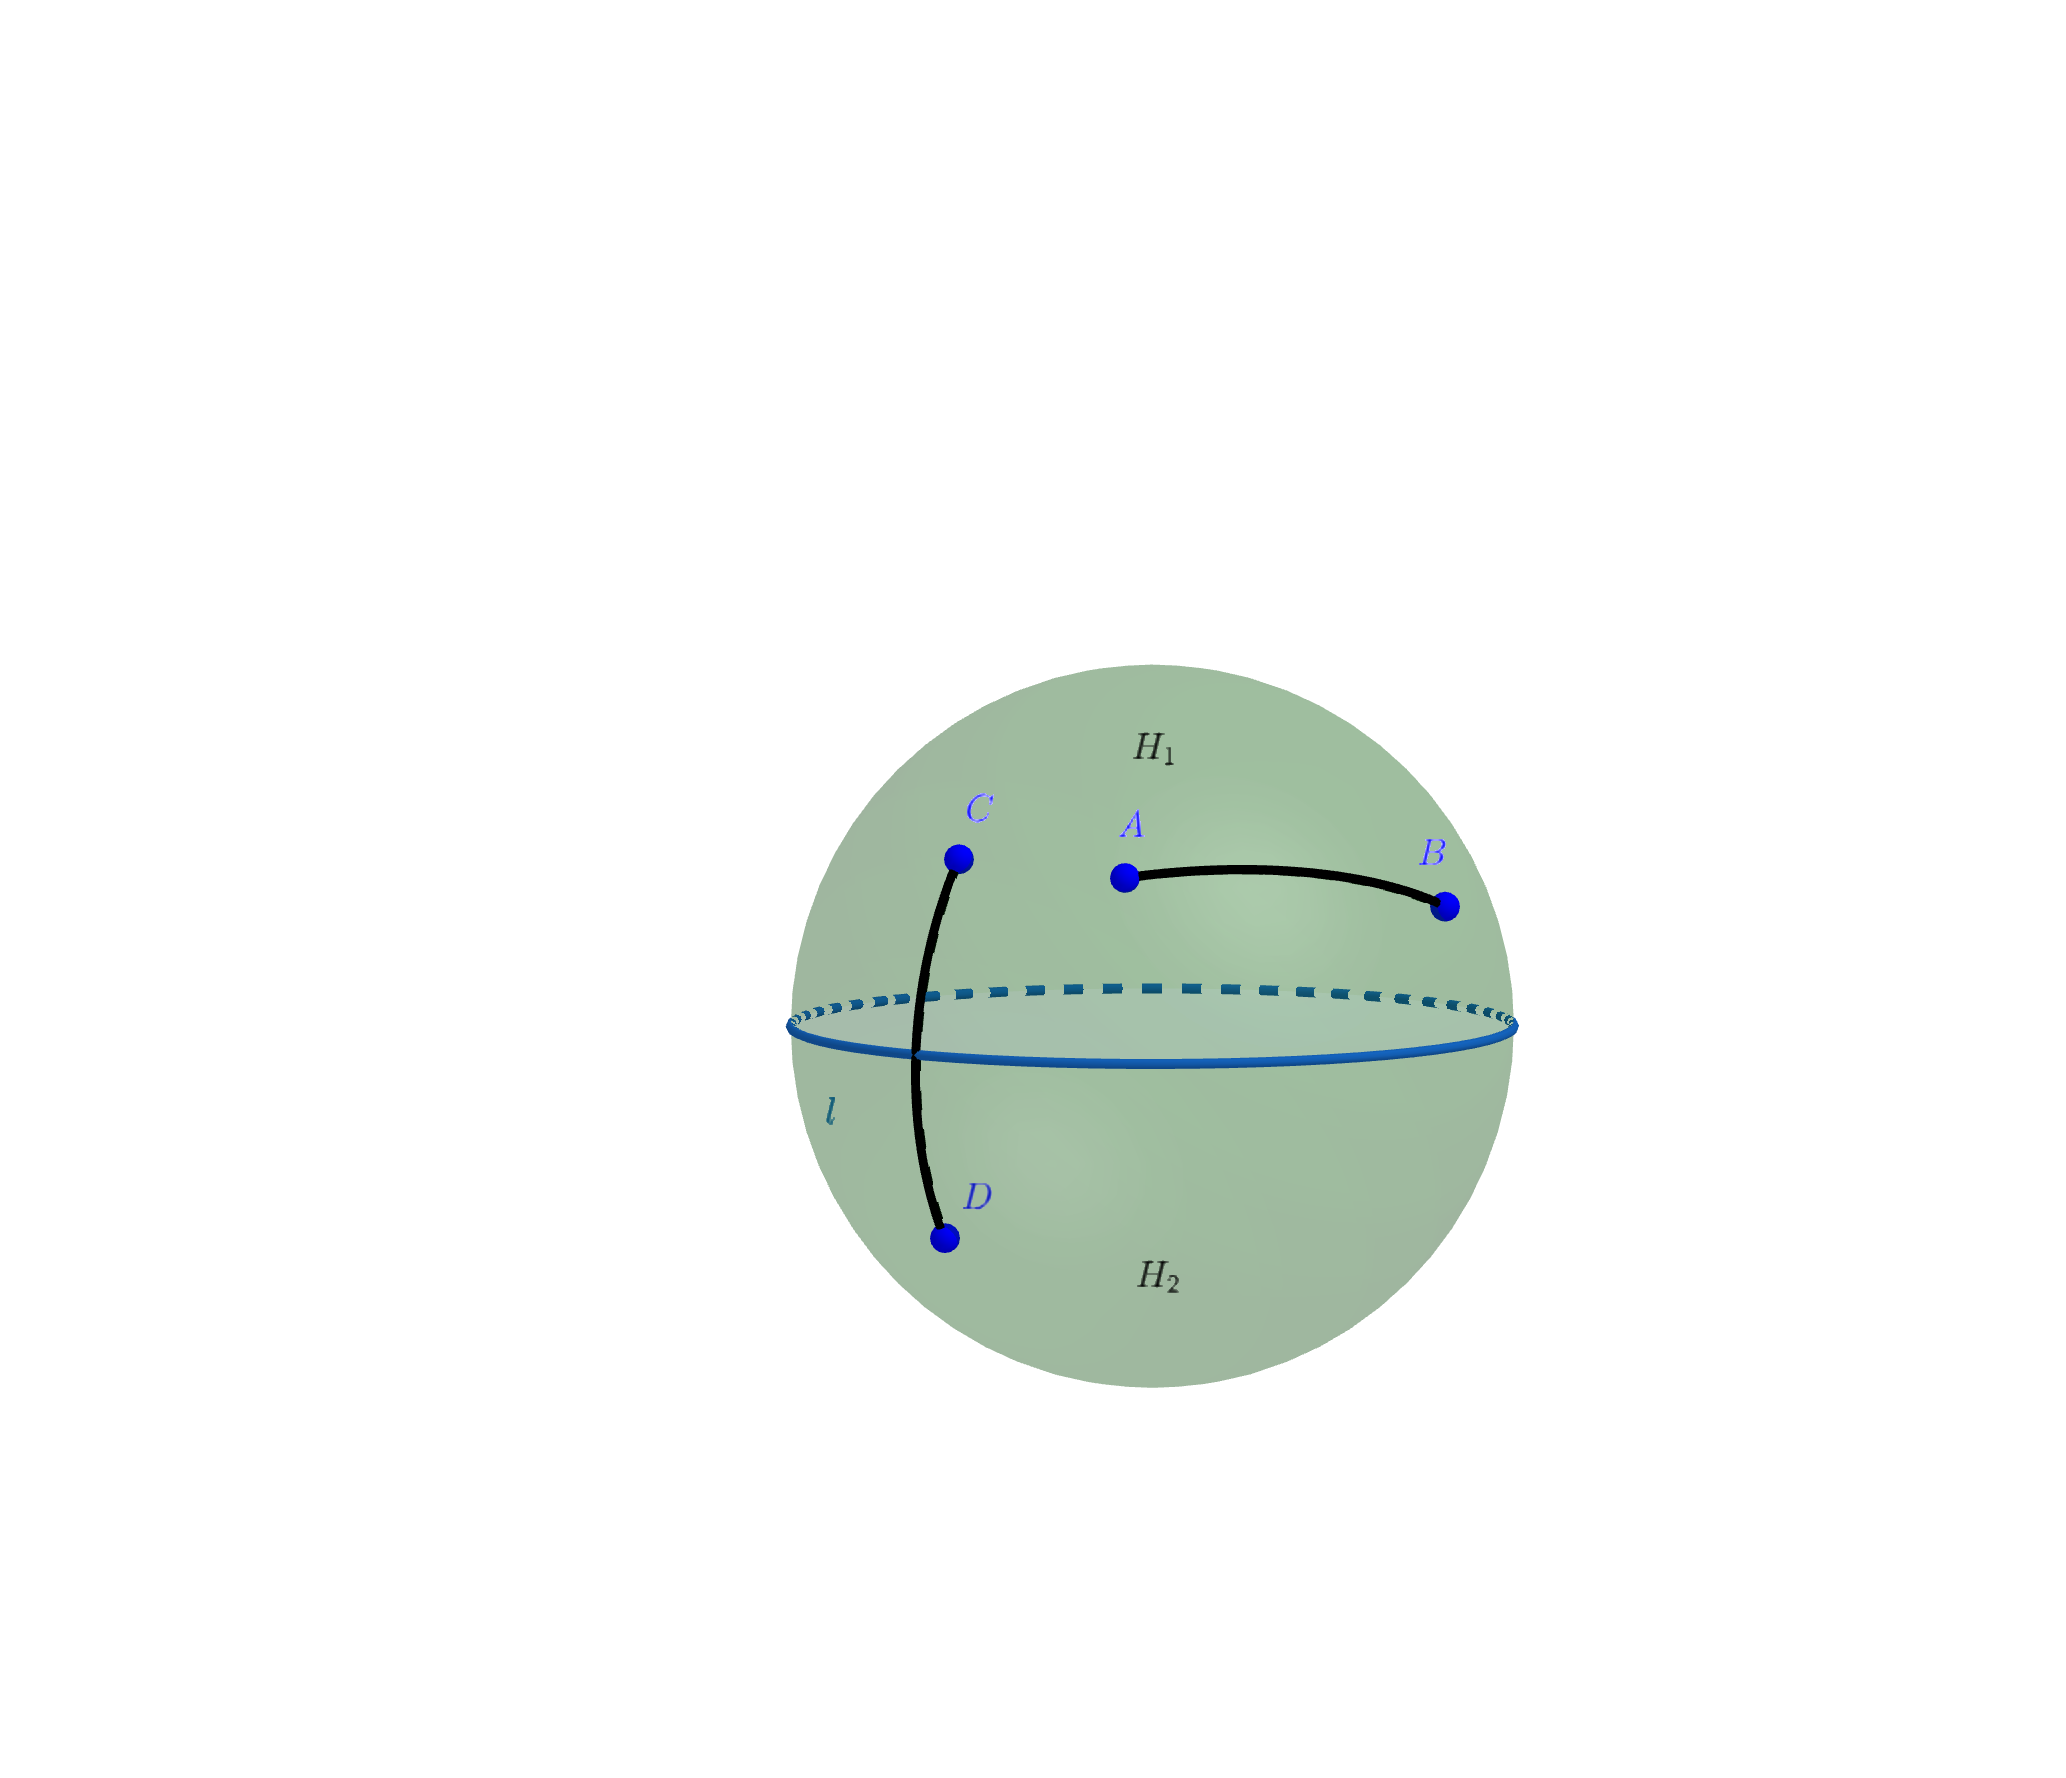
\includegraphics[trim={13cm 13cm 12cm 22cm},clip, width=0.9\textwidth]{oving_2/334a.png}
    \end{figure}
    
  \end{punkt}

  \begin{punkt}
    Vi vet fra øving 1 at $A\ast B\ast C$ hvis og bare hvis $A, B, C$ ligger på samme storsirkel og 
    $s(A, B)+s(B,C) = s(A,C)$. La nå $l$ være storsirkelen bestemt av $A$ og $B$. På en litt uformell
    måte kan vi si at $s(A, B)+s(B, C) = s(A, C)$ dersom korteste vei mellom $A$ og $C$ på storsirkelen
    $l$ går gjennom $B$. Dette skjer når $C$ ligger på den \emph{halve storsirkelen} bestemt av $A$ og 
    $B$ -- se figuren under. Merk at både $A$ og dets antipodale punkt $D$ ligger på strålen. 

    \begin{figure}[H]
      \centering 
      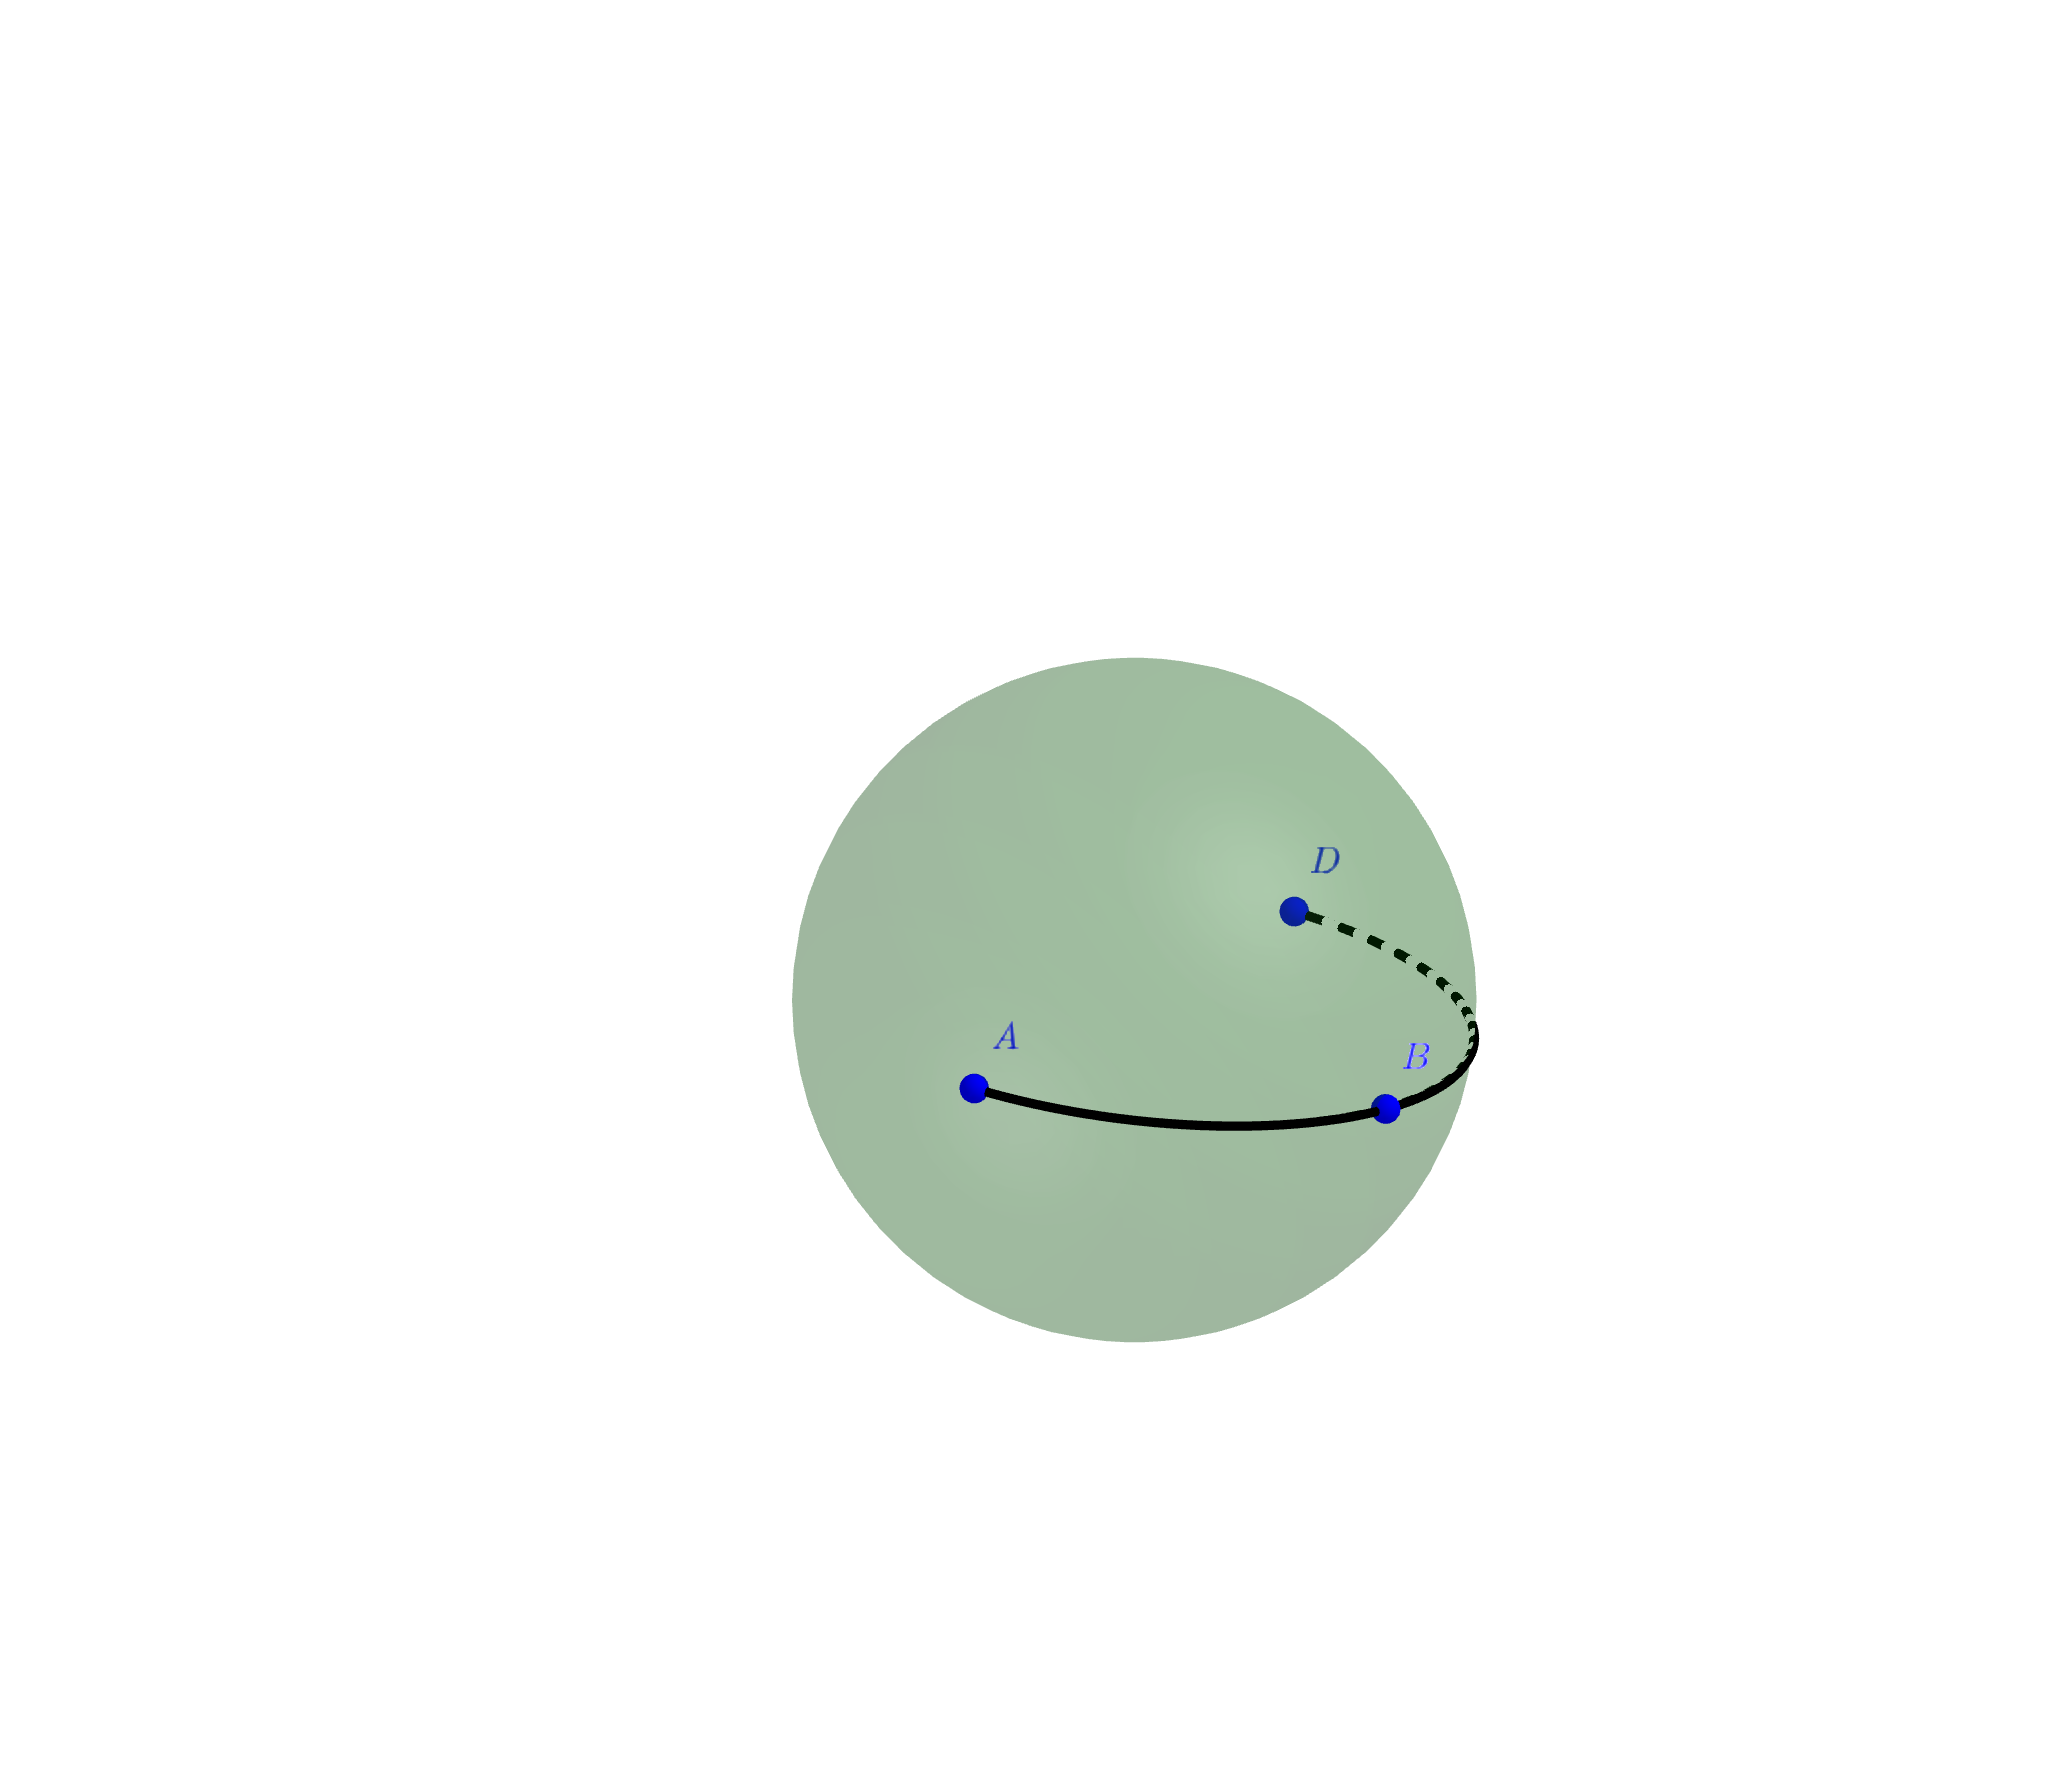
\includegraphics[trim={13cm 13cm 12cm 22cm},clip, width=0.9\textwidth]{oving_2/334b.png}
    \end{figure}
  \end{punkt}

  \begin{punkt}
    Nei, teorem 3.3.9 holder ikke her. Hvis vi lar $D$ være det antipodale punktet til $A$, ligger $D$
    på strålen $\overrightarrow{AB}$ fra deloppgave b). Men, $B$ og $D$ ligger ikke begge på en felles
    side av storsirkelen $l$, ettersom $D$ ligger \emph{på} storsirkelen $l$. Se figuren under.

    \begin{figure}[H]
      \centering 
      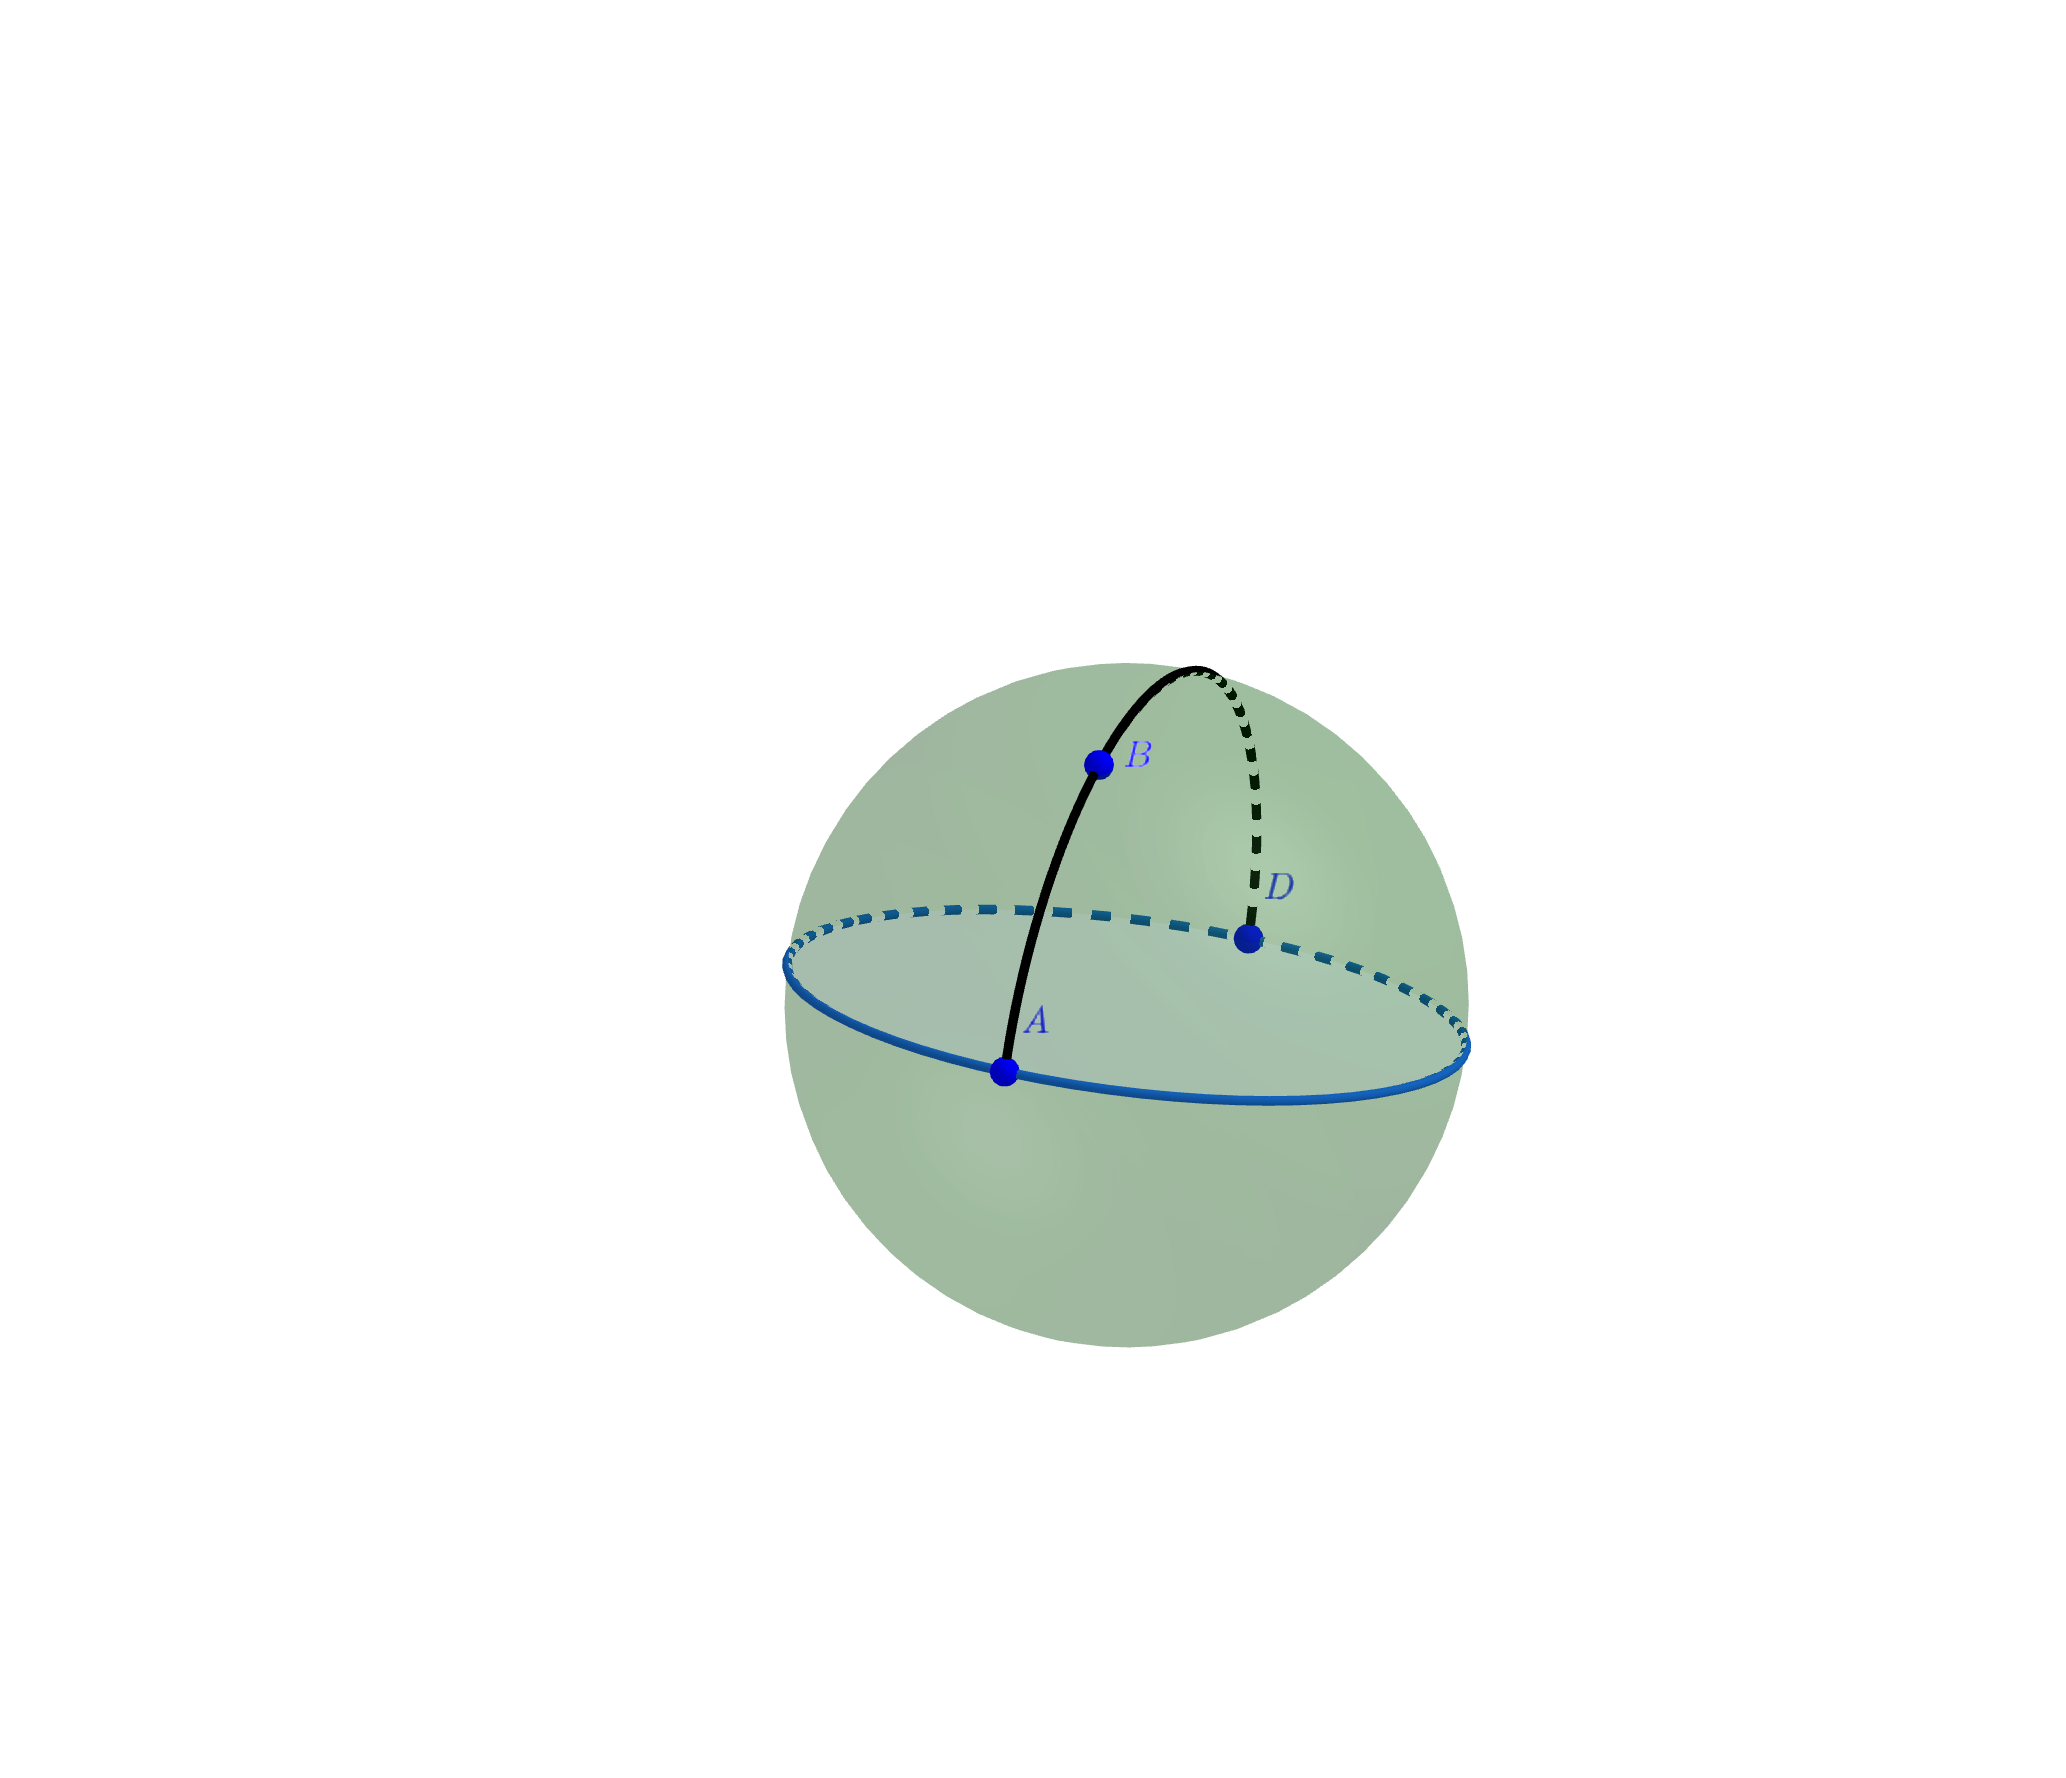
\includegraphics[trim={13cm 13cm 12cm 23cm},clip, width=0.9\textwidth]{oving_2/334c.png}
    \end{figure}
  \end{punkt}
\end{oppgave}

\begin{oppgave}[3.3.5]
  Fra planseparasjonsaksiomet deler linjen $l$ resten av planet i to halvplan $H_1$ og $H_2$. 
  Siden ingen av hjørnene $A$, $B$, $C$ ligger på $l$ må de ligge enten i $H_1$ eller 
  $H_2$. Vi har da tre punkter fordelt på to halvplan, som vil si at minst to av de må ligge i samme
  halvplan. Vi antar uten tap av generalitet at disse to punktene er $A$ og $B$, og at de ligger i 
  $H_1$. Siden $H_1$ er en konveks mengde, vil også linjestykket $\overline{AB}$ ligge i $H_1$. Dette
  betyr at ingen av punktene på $\overline{AB}$ ligger på $l$, så $l$ skjærer ikke siden $\overline{AB}$
  i trekanten. 

  Det er fult mulig for en linje å skjære trekanten $\triangle ABC$ i alle tre sidene. Linjen 
  $\overleftrightarrow{AB}$ vil skjære $\overline{AB}$ i punktet $A$, $\overline{BC}$ i punktet $B$ og 
  $\overline{AC}$ i punktet $A$. 

\end{oppgave}
 



\end{document}